% Options for packages loaded elsewhere
\PassOptionsToPackage{unicode}{hyperref}
\PassOptionsToPackage{hyphens}{url}
%
\documentclass[
  onecolumn]{article}
\usepackage{amsmath,amssymb}
\usepackage{iftex}
\ifPDFTeX
  \usepackage[T1]{fontenc}
  \usepackage[utf8]{inputenc}
  \usepackage{textcomp} % provide euro and other symbols
\else % if luatex or xetex
  \usepackage{unicode-math} % this also loads fontspec
  \defaultfontfeatures{Scale=MatchLowercase}
  \defaultfontfeatures[\rmfamily]{Ligatures=TeX,Scale=1}
\fi
\usepackage{lmodern}
\ifPDFTeX\else
  % xetex/luatex font selection
\fi
% Use upquote if available, for straight quotes in verbatim environments
\IfFileExists{upquote.sty}{\usepackage{upquote}}{}
\IfFileExists{microtype.sty}{% use microtype if available
  \usepackage[]{microtype}
  \UseMicrotypeSet[protrusion]{basicmath} % disable protrusion for tt fonts
}{}
\makeatletter
\@ifundefined{KOMAClassName}{% if non-KOMA class
  \IfFileExists{parskip.sty}{%
    \usepackage{parskip}
  }{% else
    \setlength{\parindent}{0pt}
    \setlength{\parskip}{6pt plus 2pt minus 1pt}}
}{% if KOMA class
  \KOMAoptions{parskip=half}}
\makeatother
\usepackage{xcolor}
\usepackage[margin=1in]{geometry}
\usepackage{graphicx}
\makeatletter
\newsavebox\pandoc@box
\newcommand*\pandocbounded[1]{% scales image to fit in text height/width
  \sbox\pandoc@box{#1}%
  \Gscale@div\@tempa{\textheight}{\dimexpr\ht\pandoc@box+\dp\pandoc@box\relax}%
  \Gscale@div\@tempb{\linewidth}{\wd\pandoc@box}%
  \ifdim\@tempb\p@<\@tempa\p@\let\@tempa\@tempb\fi% select the smaller of both
  \ifdim\@tempa\p@<\p@\scalebox{\@tempa}{\usebox\pandoc@box}%
  \else\usebox{\pandoc@box}%
  \fi%
}
% Set default figure placement to htbp
\def\fps@figure{htbp}
\makeatother
\setlength{\emergencystretch}{3em} % prevent overfull lines
\providecommand{\tightlist}{%
  \setlength{\itemsep}{0pt}\setlength{\parskip}{0pt}}
\setcounter{secnumdepth}{5}
\makeatletter
\renewcommand{\maketitle}{
  \onecolumn % Start in one-column mode
  \begin{center}
    {\LARGE \bfseries \@title \par}
    \vskip 1em
    {\large
      Victor Pacifique Rwandarwacu\textsuperscript{1,*}, Prof. John Newell\textsuperscript{1} \par
      \textsuperscript{1}School of Mathematical and Statistical Sciences, University of Galway, Ireland \par
      *Corresponding author: \texttt{v.rwandarwacu1@universityofgalway.ie}
    }
    \vskip 1em
    \@date
  \end{center}
  \vspace{1em}
}
\makeatother


\usepackage{subfig}
\usepackage{booktabs}
\usepackage{longtable}
\usepackage{array}
\usepackage{multirow}
\usepackage{wrapfig}
\usepackage{float}
\usepackage{colortbl}
\usepackage{pdflscape}
\usepackage{tabu}
\usepackage{threeparttable}
\usepackage{threeparttablex}
\usepackage[normalem]{ulem}
\usepackage{makecell}
\usepackage{xcolor}
\usepackage[]{natbib}
\bibliographystyle{plainnat}
\usepackage{bookmark}
\IfFileExists{xurl.sty}{\usepackage{xurl}}{} % add URL line breaks if available
\urlstyle{same}
\hypersetup{
  pdftitle={Clinicians' Interpretation and Preferences for Survival Data Visualisation: A Pre--Post Study Comparing Kaplan--Meier and Mean Residual Life Plots},
  hidelinks,
  pdfcreator={LaTeX via pandoc}}

\title{Clinicians' Interpretation and Preferences for Survival Data
Visualisation: A Pre--Post Study Comparing Kaplan--Meier and Mean
Residual Life Plots}
\author{Victor Pacifique Rwandarwacu\textsuperscript{1,*},Prof.~John
Newell\textsuperscript{1} \textbackslash{} \textsuperscript{1}School of
Mathematical and Statistical Sciences, \textbackslash{} University of
Galway, Ireland \textbackslash{} *Corresponding author:
\texttt{v.rwandarwacu1@universityofgalway.ie}}
\date{2025-06-25}

\begin{document}
\maketitle

\noindent

\rule{\linewidth}{0.4pt}

\textbf{Abstract}

Effective visualisation of survival data is key for both clinician
interpretation and patient communication. While a Kaplan Meier (KM) is a
popular and standard plot, Mean Residual Life (MRL) plots may offer a
more informed visualisation of prognosis on time scale. However, little
is known about clinicians' knowledge and preferences regarding these
alternative visualisations. In this pre--post (Pilot) cross-sectional
survey, 32 participants including medical students and doctors
voluntarily completed an online questionnaire where they were asked to
interpret four survival visualisation types (KM plot, survival
difference, MRL plot, and difference in MRL) before and after a brief
learning section. Outcomes assessed included interpretation accuracy,
learning gains, and plot preferences for clinician's understanding and
use with patients.

Overall, the pre-learning (baseline) interpretation accuracy was 50\%
{[}37.5-62.5{]}, and it was higher for the Kaplan-Meier plot than the
Mean Residual Life (MRL) plot at 56.2\% {[}37.5-71.9{]} and 43.8\%
{[}28.1-62.5{]}, respectively. Following the learning section, the
overall accuracy improved significantly to 81.2\% {[}68.8 - 92.2{]} (p =
0.002). The most significant improvement was observed for the MRL plot
(+37.5 percentage points, p = 0.010), which achieved a post-learning
accuracy of 81.2\%, similar to that of KM. Kaplan--Meier plots were the
most preferred for both ease of understanding by clinicians (59\%) and
patient communication (53\%). There was a noticeable improvement in
interpretation among participants with lower self-rated knowledge,
especially for MRL visualisation. Although KM is popular in medical
literature, MRL plots can be rapidly understood by clinicians with
minimal instruction. These findings echo the integration of MRL
visualisations into clinical dashboards and medical education to enhance
survival data communication. There is a need for large-scale study in a
controlled setting to validate these findings.

\textbf{Availability}: Code available at
\url{https://github.com/rwandarwacu1/Msc_thesis_survival}

\textbf{Keywords:} Survival analysis, mean residual life, medical data
visualisation, Kaplan--Meier, time-to-event

\noindent

\rule{\linewidth}{0.4pt}

\section{Introduction}\label{introduction}

\subsection{Background}\label{background}

Survival analysis, also referred to as time-to-event data analysis, is
the analysis of data in the form of times from a well-defined time
origin until the occurrence of some particular event or end point.
Survival analysis is a critical branch of statistics that specifically
deals with the modeling of time until an event occurs. These events may
range from biological outcomes such as death, remission, or relapse, to
engineering failures, time to default in finance, or germination in
agriculture (\citet{peaceDesignAnalysisClinical2009}). The distinct
feature of survival data is censoring, wherein the event of interest has
not been observed for all subjects during the study period. This demands
specialized statistical methods to handle incomplete observations and
skewed distributions (\citet{collettModellingSurvivalData2023};
\citet{bradburnSurvivalAnalysisPart2003}).

In medical research, survival analysis is used extensively to study
disease prognosis, treatment effectiveness, and risk prediction. The
Kaplan--Meier (KM) estimator remains one of the most commonly used tools
for visualising survival functions due to its simplicity and
non-parametric formulation
(\citet{kleinSurvivalAnalysisTechniques2006}). However, despite
widespread usage, KM plots can be difficult to interpret for individuals
without statistical background, particularly in clinical practice and
patient-centered communication contexts
(\citet{hawkinsCosteffectivenessAnalysisTreatments2005};
\citet{trevenaPresentingQuantitativeInformation2013}).

\subsubsection{Survival Function}\label{survival-function}

The survival function \(S(t)\) is the probability that the survival time
is greater than or equal to time \(t\), which is the observed value of
random variable \(T\) with distribution function \(F(t)\)
\citep{collettModellingSurvivalData2023}. It is a non-increasing
function ranging between 1 and 0.

\begin{equation}
S(t) = \mathrm{P}(T \geqslant t) = 1 - F(t) \label{eq:survival}  
\end{equation}

The cumulative distribution function is the complement of the survival
function; it gives the probability that the event has occurred by time
\(t\).

\begin{equation}
F(t) = \mathrm{P}(T < t) = \int_0^t f(u) \, \mathrm{d}u \label{eq:cumulative}
\end{equation}

The Kaplan-Meier (KM) estimator is a non-parametric method used to
estimate the survival function from observed survival times, especially
when data are censored. The resulting estimate is a stepwise
approximation of the true survival function on the probability scale,
graphically represented further in the next section.

The KM estimate of the survival function at the \(k\)-th interval is
given by: \begin{equation}
\hat{S}(t) = \prod_{j=1}^{k} \left( \frac{n_j - d_j}{n_j} \right) \label{KM estimator}
\end{equation}

For \(t_{(k)} \leqslant t < t_{(k+1)}, \ k = 1, 2, \ldots, r\), with
\(\hat{S}(t) = 1\) for \(t < t_{(1)}\), where \(t_{r+1}\) is taken to be
\(\infty\). Here, \(d_j\) denotes the number of deaths in this interval,
\(n_j\) is the number of individuals alive just before \(t_{(j)}\), and
\(d_j\) events occur at \(t_{(j)}\)
\citep{collettModellingSurvivalData2023}.

The key analytical problem in survival analysis is censoring. The most
common censoring mechanisms are right and left censoring; however, we
will focus on right censoring, which occurs when a subject has been
followed up, but the exact survival time is known to be greater than the
last follow-up time. For example, in a study in which leukemia patients
are followed until they go out of remission, if the study ends while the
patient is still in remission, then the patient's survival time is
considered censored (Administrative censoring). Moreover, censoring may
also occur when a person is lost to follow-up during the study period or
withdrawn from the study due to death or other reasons
(\citet{kleinbaumIntroductionSurvivalAnalysis2012}).

\subsubsection{Mean Residual Life (MRL)
Function}\label{mean-residual-life-mrl-function}

The MRL function estimates how much longer, on average, a subject is
expected to survive given that the subject has survived until time
\(t\).

Mathematically, the MRL function is given by : \begin{equation}
m(t) = E(T - t \mid T > t) = \frac{1}{S(t)} \int_t^\infty S(s) \, ds \label{eq:mrl}
\end{equation}

where \(T\) is survival time and \(S(t)\) the survival function.

Formula \ref{eq:mrl} demonstrates that the MRL is the area under the
survivor function beyond time \(t\), normalized by the conditional
probability of surviving beyond that point.There are various estimators,
but most of them fail for right censored data. Unlike the Kaplan--Meier
estimator for survival probabilities, MRL estimation requires a complete
understanding of the upper tail of the survival distribution. Because
censoring obscures this region, reliable estimation demands additional
assumptions or supplementary modelling,thus motivating the development
of hybrid and semi-parametric approaches.

Previous studies have suggested different hybrid approaches, especially
for parametric options in the upper tail, such as the exponential method
(\citet{suNovelMethodCalculate2012}). However, these approaches are
insufficiently flexible when the tail behavior is unknown a priori.
Notably, authors including Gelber, Goldhirsch, and Cole
(\citet{gelberParametricExtrapolationSurvival1993}), as well as Gong and
Fang (\citet{gongAsymptoticPropertiesMean2012}), have proposed the use
of goodness-of-fit procedures to guide selection of suitable parametric
models for the tail estimation. However, the selection of candidate
distributions is subject, and the large variability associated with the
Kaplan--Meier curve could compromise the choice of the appropriate
model.

To address these limitations, innovative statistical methodologies have
emerged. A hybrid semi-parametric approach proposed by Alvarez-Iglesias
et al.~(2015) leverages both non-parametric estimation for the observed
data and parametric modeling for the unobserved(censored) tail of the
survival distribution. This method conceptually divides the MRL
estimation task into two distinct components:

\begin{itemize}
 \item \textbf{Below a threshold}: The MRL is estimated non-parametrically using the Kaplan–Meier estimator. This part captures the behavior of the data that is well-supported by observed events.
 \item \textbf{Above the threshold}: The tail of the survival function is modeled using extreme value theory (EVT), specifically by fitting a Generalized Pareto Distribution (GPD) to the excess times.
\end{itemize}

This combination addresses the issue of right-censoring by extrapolating
the survival distribution beyond the last observed time point, using a
model justified by the Extreme Value Theory (EVT).

The GPD is selected for its flexibility---it encompasses a range of tail
behaviors from light (e.g.,exponential) to heavy-tailed distributions.
Its defining parameters, the scale \(\sigma\) and shape \(\xi\), are
estimated via maximum likelihood using the observed data above the
threshold \(u\). Importantly, EVT provides theoretical justification for
using the GPD in this setting, ensuring that the extrapolation is
statistically valid under broad conditions.

The threshold plays a critical role. It should be high enough to ensure
that the EVT approximation holds, but low enough to retain sufficient
data for stable estimation. Diagnostic tools or quantile-based
heuristics (e.g., the 80th percentile of observed uncensored times) are
frequently employed to guide this selection.

\paragraph{Description of hybrid semi-parametric
method}\label{description-of-hybrid-semi-parametric-method}

Let \(T\) be the true survival time and let \(C\) be the censoring time,
and assume that \(T\) and \(C\) are independent.

For an individual \(i\), the observed pair is \((X_i, \delta_i)\), where
\(X_i = \min(T_i, C_i)\) and \(\delta_i = I_{T_i < C_i}\).

Let \(\{(x_1, \delta_1), (x_2, \delta_2), \dots, (x_n, \delta_n)\}\) be
a random sample of observed times and censoring indicators.

Let \(T^*\) be the maximum observed time. The estimate of the Mean
Residual Life (MRL) function at time \(t\), denoted \(\hat{m}(t)\), is
obtained as follows:

\begin{enumerate}
\def\labelenumi{\arabic{enumi}.}
\tightlist
\item
  Choose a threshold \(u\) and select the observations \(\xi\) that are
  between \(u\) and \(T^*\). Let \(m\) denote the number of these
  observations.
\item
  Calculate the maximum likelihood estimates of the parameters \(\xi\)
  and \(\sigma_u\) of the Generalized Pareto Distribution (GPD) using
  the \(m\) observations that are between \(u\) and \(T^*\). The
  censored likelihood function is
\end{enumerate}

\begin{equation}
L(\xi, \sigma_u; t_i, \delta_i) = \prod_{i=1}^{m} \left( \frac{1}{\sigma_u} \left[ 1 + \frac{\xi t_i}{\sigma_u} \right]^{-1/\xi} \right)^{\delta_i} \left( \left[ 1 + \frac{\xi t_i}{\sigma_u} \right]^{-1/\xi} \right)^{1 - \delta_i} \label{eq:likelihood}
\end{equation}

where \(t_i\) are the excesses above the threshold \(u\), that is,
\(t_i = x_i - u\). This function can be maximized using standard
optimization methods.

\begin{enumerate}
\def\labelenumi{\arabic{enumi}.}
\setcounter{enumi}{2}
\tightlist
\item
  Estimate the restricted MRL below \(u\) using the Kaplan-Meier
  estimator. This estimate will be called \(\hat{m}_{\text{KM}}(t)\).
\item
  Estimate MRL at time \(u\) for the GPD:
\end{enumerate}

\begin{equation}
\hat{m}(u) = \frac{\hat{\sigma}_u}{1 - \hat{\xi}} \label{eq:mrl_u}
\end{equation}

where \(\hat{\xi}\) and \(\hat{\sigma}_u\) are the maximum likelihood
estimates from step 2.

\begin{enumerate}
\def\labelenumi{\arabic{enumi}.}
\setcounter{enumi}{4}
\tightlist
\item
  Finally, the full MRL estimate at any time \(t\) is obtained by
  summing the estimated area under the Kaplan--Meier curve from \(t\) to
  \(u\), and the area under the extrapolated tail from \(u\) to
  infinity, weighted by survival probabilities:
\end{enumerate}

\begin{equation}
\hat{m}(t) = \hat{m}_{\text{KM}}(t) + \hat{m}(u) \cdot \frac{\hat{S}_{\text{KM}}(u)}{\hat{S}_{\text{KM}}(t)} \label{eq:mrl_total}
\end{equation}

This method allows for a smooth and interpretable estimation of the MRL,
even when censoring prevents direct estimation using classical
techniques.

\subsection{Example dataset}\label{example-dataset}

The dataset used to generate figure 1 to 4 was drawn from the Cancer
Genome Atlas -- Breast Cancer (TCGA-BRCA) database, a well-curated, open
access repository of longitudinal survival and clinical data
(\citet{CancerGenomeAtlas}).

To simulate realistic clinical subgroup comparisons, subjects were
stratified based on binary pathological stages. The plot types were
constructed using R and later used in the survey for interpration and
ranking by clinicians which is further discussed in Methodology section.
Generated plots include :

\begin{itemize}
\item \textbf{Kaplan-Meier (KM) plot}: Stepwise curve showing estimated survival probability over time
\item \textbf{Survival difference plot}: Curve showing pointwise difference in survival probabilities between groups. 
The survival difference between two groups \( A \) and \( B \) at time \( t \) is given by:

\begin{equation}
\Delta S(t) = S_A(t) - S_B(t)
\label{eq:survival_difference}
\end{equation}

Where:
 \( S_A(t) \) is the survival function for group \( A \),
 \( S_B(t) \) is the survival function for group \( B \).
\item \textbf{Mean Residual Life (MRL) plot}: Mean residual life at time t; expected remaining lifespan given survival to t
\item \textbf{Difference in Mean Residual Life (MRL) plot} : Difference in MRL estimates between two groups over time
\end {itemize}

MRL plots were estimated using a hybrid semi parametric method proposed
by \citet{alvarez-iglesiasSummarisingCensoredSurvival2015a}

\begin{figure}[H] \centering
\begin{minipage}[b]{0.45\textwidth} 
\centering 
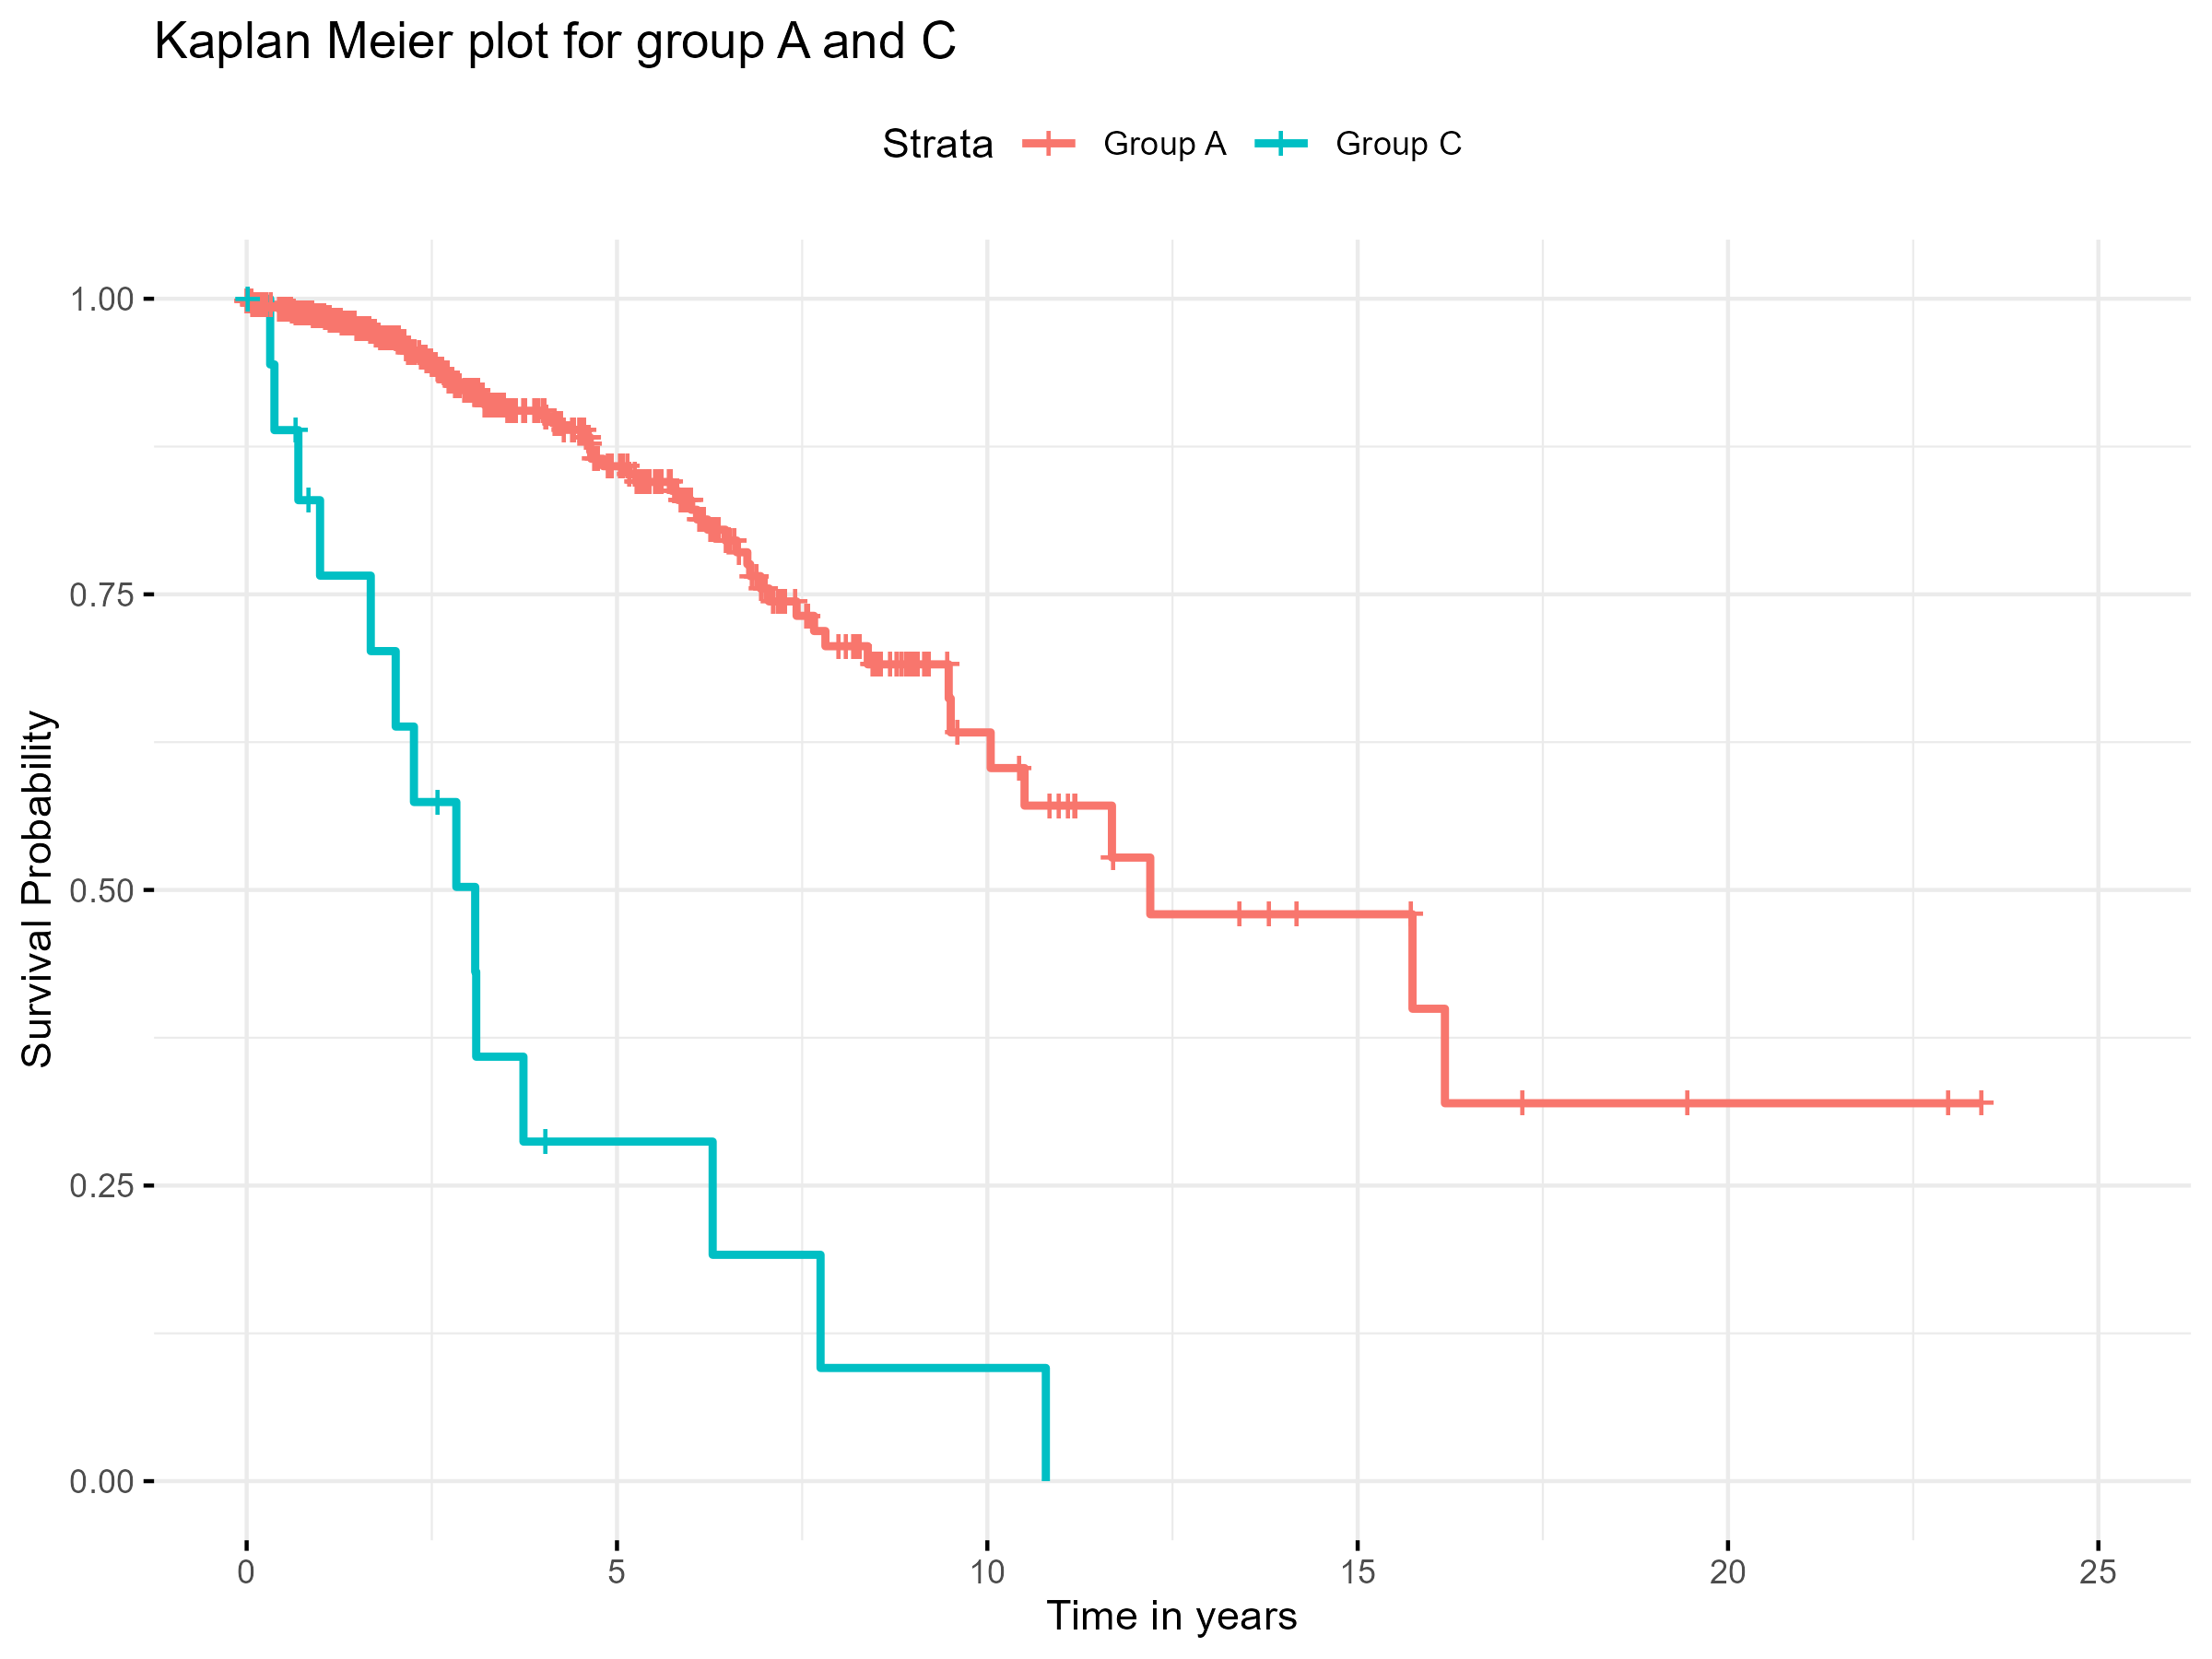
\includegraphics[width=1.0\textwidth]{KM_Example.png} 
\caption{Kaplan Meier plot} 
\end{minipage}
\begin{minipage}[b]{0.45\textwidth} 
\centering 
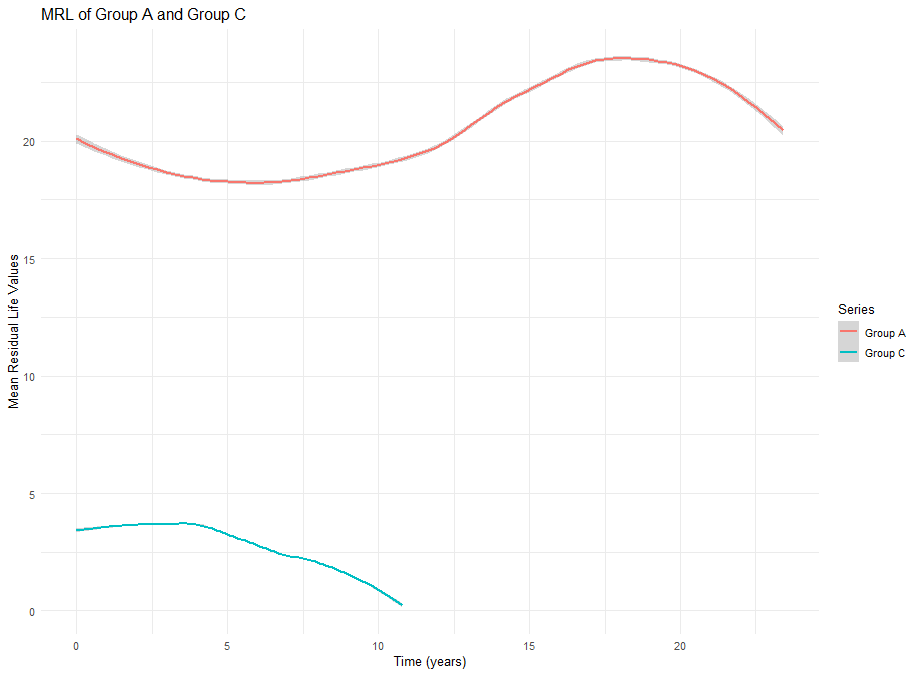
\includegraphics[width=1.0\textwidth]{MRL Example.jpeg} 
\caption{Mean Residual Life plot} 
\end{minipage}
\vspace{1em}
\begin{minipage}[b]{0.45\textwidth} 
\centering 
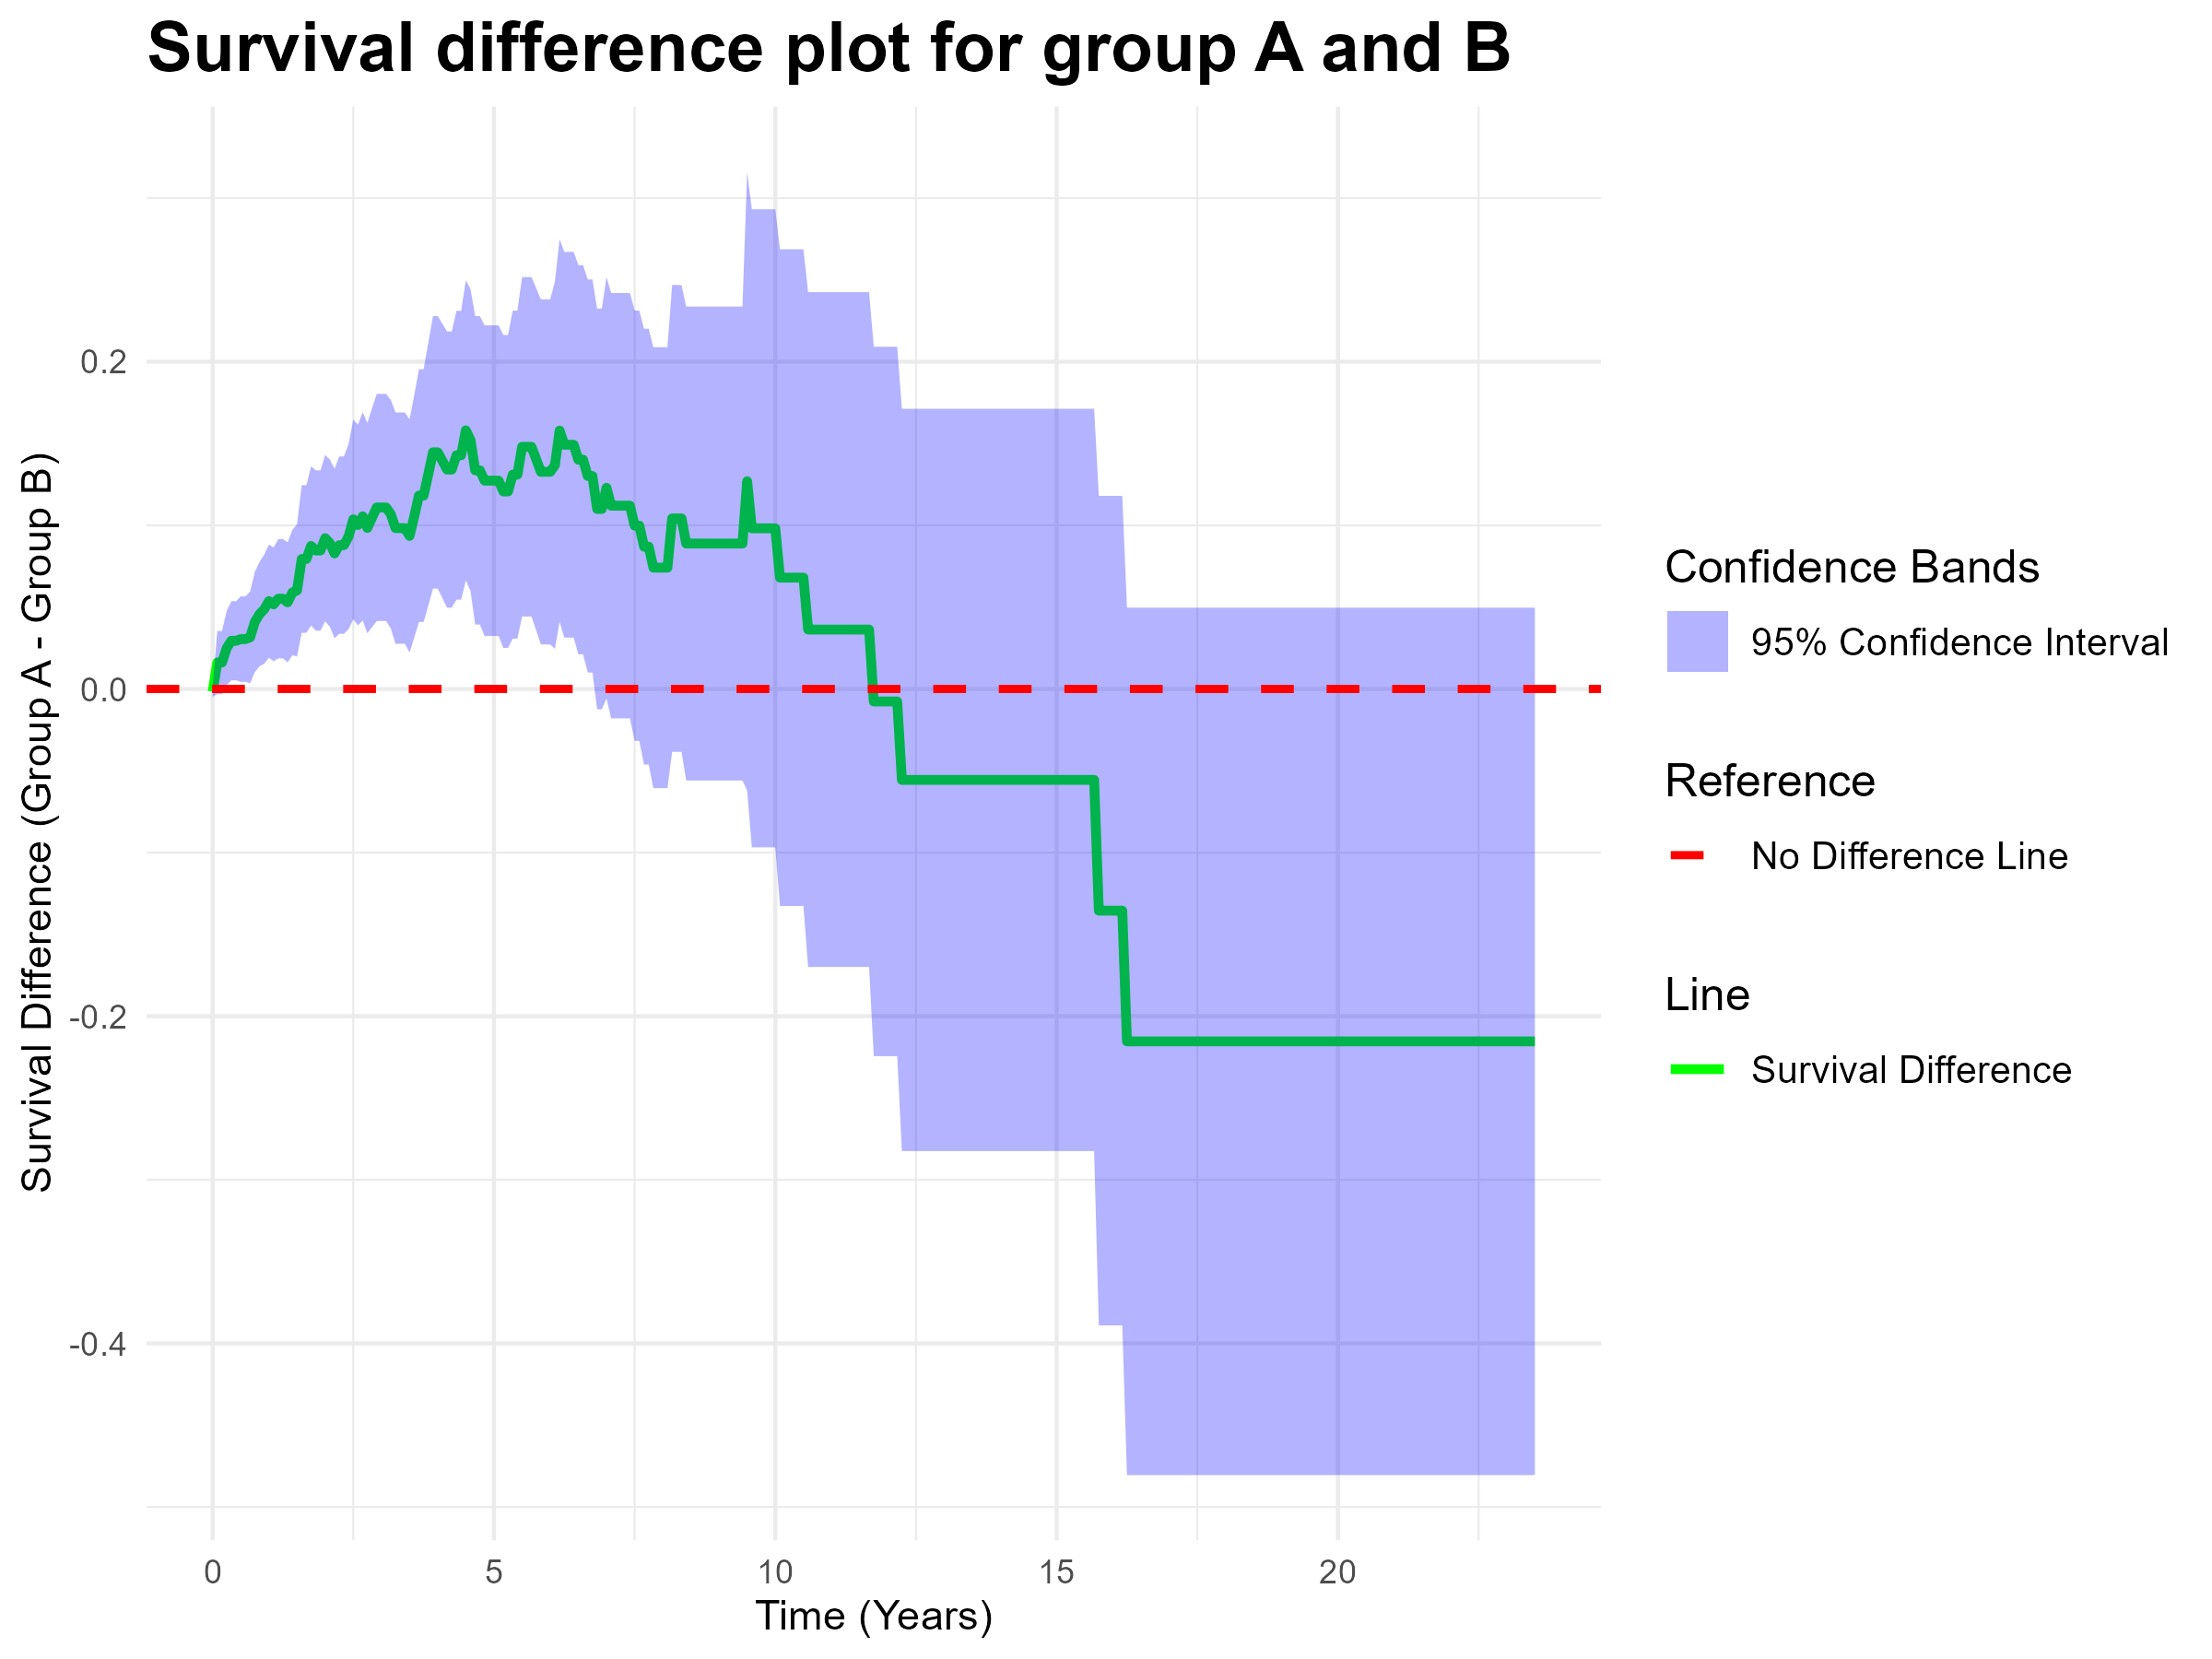
\includegraphics[width=1.0\textwidth]{Example survival diff.png} 
\caption{Difference in survival plot} 
\end{minipage}
\begin{minipage}[b]{0.45\textwidth} 
\centering 
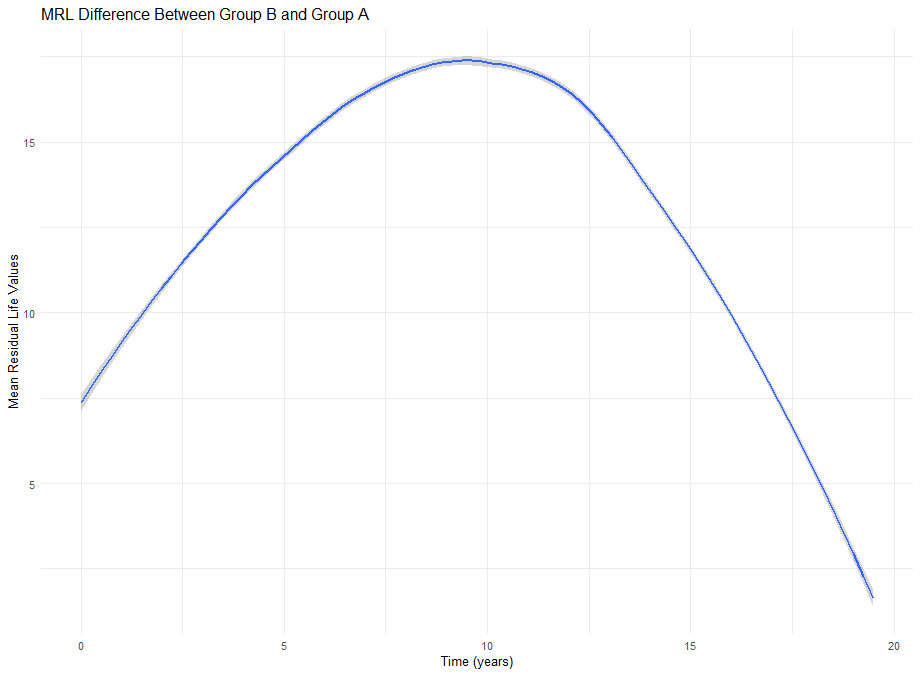
\includegraphics[width=1.0\textwidth]{Example MRL Diff.jpeg} 
\caption{Difference in MRL plot} 
\end{minipage}
\end{figure}

\subsection{Survival Visualisation}\label{survival-visualisation}

While KM and survival difference plots are informative, they operate on
a probability scale, which may not resonate intuitively with human
perceptions of remaining lifespan or life expectancy
(\citet{spiegelhalterVisualizingUncertaintyFuture2011}). This limitation
is especially relevant when clinicians need to translate survival
statistics into terms understandable by patients, such as ``How much
longer can I expect to live?''
(\citet{pencinaPredicting30YearRisk2009}).

The Mean Residual Life (MRL) function is a valuable alternative in such
scenarios. Unlike survival probabilities or hazard rates, MRL explicitly
quantifies prognosis in time units, which may better support clinical
interpretation and patient discussions
(\citet{wangNonparametricSemiparametricEstimation2017};
\citet{wangReslifeResidualLifetime2023}). The hybrid estimator discussed
herein presents a flexible yet theoretically grounded framework for
estimating MRL in the presence of censoring and has been implemented in
practical tools such as interactive Shiny web applications designed for
translational statistics
(\citet{albertoalvarez-iglesiasOnlineTranslationalTool};
\citet{amirhosseinjalaliTranslationalStatisticsDynamic2018}).

For the graphical comparison of time-to-event outcomes across different
groups, survival difference, and survival ratio plots are the most
popular alternatives. The survival ratio plot, in particular,facilitates
the identification of temporal windows during which survival outcomes
diverge between distinct populations or interventions. Using resampling
techniques, permutation envelopes are generated as reference bands to
investigate whether the observed differences reflect true effects or
arise from random variation is due to sampling variation or a possible
real effect (\citet{newellSurvivalRatioPlots2006c}). Nonetheless, these
visualisations continue to express outcomes on the probability scale.

The survival ratio between two groups \(A\) and \(B\) at time \(t\) is
given by:

\begin{equation}
\text{Survival Ratio}(t) = \frac{S_A(t)}{S_B(t)}
\label{eq:survival_ratio}
\end{equation}

where: \(S_A(t)\) is the survival function for group \(A\), \(S_B(t)\)
is the survival function for group \(B\).

The consensus study on visualising harm in clinical trials suggested the
top most recommended plot across diverse data categories, including
binary, etc., and specifically for time to event data, Kaplan Meier,
survival ratio plot, and mean cumulative plots were the only recommended
options (\citet{phillipsVisualisingHarmsPublications2022}) . The mean
residual life plot did not figure among the top choices.

Sengupta (\citet{senguptaGraphicalToolsCensored1995}) has emphasized the
importance of improved graphical representations for censored survival
data, advocating for more intuitive visual tools that can bridge the gap
between quantitative accuracy and clinical usability.

Notably, the relevance of MRL visualizations has been explored in
various health-related domains, including oncology, transplant medicine,
and infectious disease prognosis
(\citet{achilonuModellingGraftSurvival2017};
\citet{qayoomDevelopmentNovelExtension2025}). However, it is rarely used
in clinical settings
(\citet{alvarez-iglesiasSummarisingCensoredSurvival2015a}), and the
actual interpretation and preference patterns among
clinicians---particularly when exposed to both traditional and MRL-based
plots---remain under-explored.

\subsection{Clinician Interpretation and Communication
Gaps}\label{clinician-interpretation-and-communication-gaps}

As the healthcare sector increasingly embrance digital transformation
data-driven decision-making, there is a pressing need to ensure that the
output of sophisticated statistical models is both interpretable and
actionable by frontline clinicians
(\citet{belangerSharedDecisionmakingPalliative2011}), which aligns with
the translational statistics concept, which encourages the dissemination
of statistical findings in a manner that clinicians with a limited
statistical background can easily grasp and apply
(\citet{mccabeArtTranslationalStatistics2022a}). Despite substantial
advances in modeling, the usability of survival plots in real-world
clinical communication remains limited
(\citet{coxSurvivalAttributableExposure2009}). Poor comprehension of
survival data can hinder patient counseling, risk stratification, and
even shared decision-making
(\citet{trevenaPresentingQuantitativeInformation2013}).

There is increasing acknowledgement that MRL plots, by shifting the
focus from probabilities to remaining life expectancy, could be a better
communication tool. Yet, formal assessment of their interpretability,
preference, and perceived usefulness among medical practitioners has not
been rigorously conducted in the literature.

\subsection{Objectives of the study}\label{objectives-of-the-study}

This study aims to assess the baseline knowledge of medical students and
doctors on survival plot interpretation and how their comprehension
evolves post-learning. It also compares MRL visualisations with
conventional survival analysis plots, specifically Kaplan Meier curves,
in terms of interpretation accuracy and clinician preferences for
communicating prognosis to patients.

\section{Methods}\label{methods}

\subsection{Study design overview}\label{study-design-overview}

This is a mixed methods study. This pilot study adopted a pre--post
learning cross-sectional survey design to assess how medical doctors and
students interpret and evaluate various visualisations of time-to-event
data including Kaplan--Meier (KM), Mean Residual Life (MRL) plots. The
survey was deployed using an online Google Form, accessible via both
mobile and desktop devices, and was open for responses over a period of
six weeks.

\subsection{Participants and
Recruitment}\label{participants-and-recruitment}

Eligible participants included medical students and doctors. The study
imposed no restrictions based on geographical location or medical
specialty. The recruitment was carried through convenience sampling,
using professional groups Social media platforms targeting health
professionals.

Participation was entirely voluntary, and no incentives were offered. A
total of 32 complete responses were included in the final analysis after
excluding incomplete submissions. Ethical approval was not required for
this pilot study.

\subsection{Survey structure}\label{survey-structure}

The structured questionnaire had five sections :

\begin{itemize}
\item \textbf{(1)} Demographic and self rated score survival knowledge: Participants were asked to report their country of medical training,level of clinical training and self-assessed familiarity with survival analysis (Likert scale 1 to 10).
\item \textbf{(2)} Pre learning (baseline) plot interpretation: Participants were shown four distinct survival visualisations and asked to provide brief written interpretations. This  section aimed to assess their baseline understanding. 
\item \textbf{(3)} Learning section: The correct interpretations were provided for the plots given in section 2.
\item \textbf{(4)} Post-learning plot(test) interpretation: Respondents were given a new set of plots, similar in format but based on different data. They were asked to answer the same interpretation questions as before,
enabling comparison of pre- and post-learning accuracy. 
\item \textbf{(5)} Ranking visualisations:Participants ranked the plots for easy interpretability by clinicians (themselves) and use for patient communication in consultation.

\end{itemize}

\subsection{Statistical Analysis}\label{statistical-analysis}

Each interpretation response was scored as correct or incorrect basing
on respondent's ability to identify visually a group with better
survival. Accuracy score was calculated per plot and per participant for
both the pre- and post-learning phases, focusing specifically on Kaplan
Meier and MRL plot. To assess the statistical significance of changes in
accuracy post learning section, Paired McNemar's tests were applied.
Descriptive statistics were used to summarise participant demographics,
self-reported knowledge levels, and ranking outcomes. Learning gain was
calculated as the percent increase in correct interpretation per
participant.

Exploratory regression tree analysis was used to identify predictors
associated with greater improvement among pre-learning score,
qualification, and self rated knowledge. Moreover, classification tree
was fitted to examine variables associated with accurate interpretation
of MRL plot post learning, representing the novel visualisation under
evaluation.

NVivo was used to code correct and incorrect interpretations and then R
for complete data analysis, visualizations by ggplot2 library,
statistical tests and ranking summaries.

\subsection{Outcome measures}\label{outcome-measures}

This study assessed interpretation accuracy, learning gain, and Plot
ranking for clinician ease of understanding and patient education. It
also explored the predictors of improvement in the post-learning
section.

\section{Results}\label{results}

\subsection{Participants
characteristics}\label{participants-characteristics}

A total of 32 participants from nine countries completed the survey. The
most common country of medical training was Rwanda (62.5\%), followed by
Ireland (9.4\%) and Switzerland (9.4\%). The majority of participants
were either medical doctors with specialty training or residents
(46.9\%) or general practitioners (43.8\%) (Table
\ref{tab:respondents}).

\begin{table}

\caption{\label{tab:tab1}Respondents’ characteristics \label{tab:respondents}}
\centering
\begin{tabular}[t]{ll}
\toprule
  & Overall\\
\midrule
 & (N=32)\\
\addlinespace[0.3em]
\multicolumn{2}{l}{\textbf{Country}}\\
\hspace{1em}Ethiopia & 2 (6.3\%)\\
\hspace{1em}Germany & 1 (3.1\%)\\
\hspace{1em}Ireland & 3 (9.4\%)\\
\hspace{1em}Italy & 1 (3.1\%)\\
\hspace{1em}Portugal & 1 (3.1\%)\\
\hspace{1em}Rwanda & 20 (62.5\%)\\
\hspace{1em}Spain & 1 (3.1\%)\\
\hspace{1em}Switzerland & 3 (9.4\%)\\
\addlinespace[0.3em]
\multicolumn{2}{l}{\textbf{Self\_reported\_Knowledge}}\\
\hspace{1em}Mean (SD) & 4.09 (2.37)\\
\hspace{1em}Median [Min, Max] & 4.00 [1.00, 9.00]\\
\addlinespace[0.3em]
\multicolumn{2}{l}{\textbf{Qualification}}\\
\hspace{1em}Medical Doctor (General Practitioner) & 14 (43.8\%)\\
\hspace{1em}Medical Doctor (Specialist or postgraduate) & 15 (46.9\%)\\
\hspace{1em}Medical student & 3 (9.4\%)\\
\bottomrule
\end{tabular}
\end{table}

Participants self-rated their prior knowledge of survival analysis with
a mean of 4.09 (SD = 2.37) on a 10-point Likert scale, with a median of
4. As shown in Figure \ref{fig2}, 75\% of respondents rated their
knowledge five or less, indicating generally limited prior familiarity
with survival methods.

\begin{figure}

{\centering 
\includegraphics[width=0.8\linewidth]{Thesis_Manuscript_Victor---arXiv--draft-_files/figure-latex/fig2-1} 

}

\caption{\label{fig2}Distribution of self-rated knowledge scores for survival analysis: 5 and 1 are the most frequent score,  7 and 6 respectively. }\label{fig:fig2}
\end{figure}

\subsection{Overall Interpretation
Accuracy}\label{overall-interpretation-accuracy}

At baseline, the overall pre-learning interpretation accuracy for KM and
MRL plots was 50.0\% (95\% CI {[}37.5 - 62.5{]}). Figure \ref{fig3}
illustrates the relationship between self-rated knowledge of survival
analysis (mean = 4.09) and pre-learning accuracy. Participants with
higher self-rated knowledge (above five) have comparable performance to
those with lower self-rated knowledge (below five). However, those with
the lowest self-rated knowledge, 1/10, have the lowest score, 25\%.

Following the learning section, post-learning accuracy improved
significantly to 81.2\% (95\% CI {[}68.8 - 92.2{]}). This represents a
mean learning gain of +31.2 percentage points (95\% CI {[}15.6 -
46.9{]}), which was statistically significant (Wilcoxon signed-rank
test, p = 0.002), as shown in Figure \ref{fig4} and Table
\ref{tab:overall}. These results indicate that the brief learning
exercise was effective in improving participants' ability to interpret
survival visualisations.

\begin{figure}

{\centering 
\includegraphics[width=0.8\linewidth]{Thesis_Manuscript_Victor---arXiv--draft-_files/figure-latex/fig3-1} 

}

\caption{\label{fig3}Proportion of Correct Interpretation per Self-rated Knowledge}\label{fig:fig3}
\end{figure}

\begin{figure}

{\centering 
\includegraphics[width=0.8\linewidth]{Thesis_Manuscript_Victor---arXiv--draft-_files/figure-latex/fig4-1} 

}

\caption{\label{fig4}Overall Proportion of Correct Interpretations (with 95\% CI), }\label{fig:fig4}
\end{figure}

\begin{figure}

{\centering 
\includegraphics[width=0.8\linewidth]{Thesis_Manuscript_Victor---arXiv--draft-_files/figure-latex/fig5-1} 

}

\caption{\label{fig5}Proportion of Correct Interpretations (Pre vs Post Learning) by plot}\label{fig:fig5}
\end{figure}

\subsection{Improvement in Interpretation accuracy per Plot
Type}\label{improvement-in-interpretation-accuracy-per-plot-type}

Interpretation improvements varied across both KM and MRL plots, as
demonstrated in Figure \ref{fig5}, and Figure \ref{fig6}, and summarised
in Table \ref{tab:outcomes}. Kaplan--Meier plots, which were the most
familiar to participants, showed an improvement in accuracy from 56.2\%
pre-learning to 81.2\% post-learning, equivalent to a gain of 25.0
percentage points (p = 0.027). The novel MRL plot showed an improvement,
with accuracy increasing from 43.8\% to 81.2\%, representing a
substantial gain of 37.5 percentage points (p = 0.010).

An alluvial diagram (Figure \ref{fig6}) illustrates the transitions in
interpretation accuracy for both plot types. The most shifts from
incorrect to correct interpretations were observed for the MRL plot,
reflecting the impact of the learning section on an individual level and
indicating a positive learning effect.

\begin{figure}

{\centering 
\includegraphics[width=0.8\linewidth]{Thesis_Manuscript_Victor---arXiv--draft-_files/figure-latex/fig6-1} 

}

\caption{\label{fig6}Alluvial Diagram of Changes in Interpretation per Plot Type}\label{fig:fig6}
\end{figure}

\begin{table}[!h]
\centering
\caption{\label{tab:tab2 }Overall Summary of Key Outcomes (with 95\%  CIs, Wilcoxon p-value)\label{tab:overall}}
\centering
\resizebox{\ifdim\width>\linewidth\linewidth\else\width\fi}{!}{
\begin{tabular}[t]{lc}
\toprule
Metric & Overall\\
\midrule
\cellcolor{gray!10}{Pre-learning accuracy} & \cellcolor{gray!10}{50.0\% [37.5 - 62.5]}\\
Post-learning accuracy & 81.2\% [68.8 - 92.2]\\
\cellcolor{gray!10}{Learning gain (points)} & \cellcolor{gray!10}{+31.2 [15.6 - 46.9]}\\
Learning gain p-value (Wilcoxon) & p = 0.002\\
\bottomrule
\end{tabular}}
\end{table}

\begin{table}[!h]
\centering
\caption{\label{tab:tab3 }Summary of Key Outcomes (with 95\%  CIs) Per Plot \label{tab:outcomes}}
\centering
\resizebox{\ifdim\width>\linewidth\linewidth\else\width\fi}{!}{
\begin{tabular}[t]{lcc}
\toprule
Metric & KM Plot & MRL Plot\\
\midrule
\cellcolor{gray!10}{Pre-learning accuracy} & \cellcolor{gray!10}{56.2\% [40.6 - 75.0]} & \cellcolor{gray!10}{43.8\% [28.1 - 62.5]}\\
Post-learning accuracy & 81.2\% [68.8 - 93.8] & 81.2\% [68.8 - 93.8]\\
\cellcolor{gray!10}{Learning gain (points)} & \cellcolor{gray!10}{+25.0 [9.4 - 43.8]} & \cellcolor{gray!10}{+37.5 [15.6 - 59.4]}\\
Learning gain p-value & p = 0.027 & p = 0.01\\
\cellcolor{gray!10}{Top-ranked for ease to communicate to patients} & \cellcolor{gray!10}{53\%} & \cellcolor{gray!10}{9\%}\\
\addlinespace
Top-ranked for ease of understanding by  clinicians & 59\% & 6\%\\
\bottomrule
\end{tabular}}
\end{table}

\subsection{Learning Gain Among Participants with Lower Self-Rated
Knowledge}\label{learning-gain-among-participants-with-lower-self-rated-knowledge}

The effect of the learning section was more pronounced among
participants with lower self-rated knowledge of survival analysis.
Figure \ref{fig7} shows that participants who rated their prior
knowledge below 5 achieved significant improvement, especially in
interpreting MRL plots. This finding highlights that even clinicians and
students with limited statistical knowledge can rapidly improve their
understanding of advanced survival visualisations when provided with
well-suited materials and contexts.

\begin{figure}

{\centering 
\includegraphics[width=0.8\linewidth]{Thesis_Manuscript_Victor---arXiv--draft-_files/figure-latex/fig7-1} 

}

\caption{\label{fig7}Learning Gain for Low-Knowledge Respondents: Overall there is remarkable gain post learning section}\label{fig:fig7}
\end{figure}

\subsection{Exploratory Analysis of predictors of
Accuracy}\label{exploratory-analysis-of-predictors-of-accuracy}

Regression tree analysis (Figure \ref{fig8}) identified the pre-learning
total correct score and participant qualification, such as being a
medical specialist or student, as key predictors of overall learning
gain among the respondents. In general, participants with lower baseline
scores demonstrated greater improvement following the learning section.

Figure \ref{fig9} further illustrates that a combination of higher
self-rated knowledge and qualification status best predicted
post-learning accuracy for the novel MRL plot. Participants with high
self-rated scores and general practitioners were more likely to achieve
higher interpretation accuracy for MRL plots in the post-learning
section, underscoring the accessibility of MRL visualisations when
supported by structured learning in both clinical and academic settings.

\begin{figure}

{\centering 
\includegraphics[width=0.8\linewidth]{Thesis_Manuscript_Victor---arXiv--draft-_files/figure-latex/fig8-1} 

}

\caption{\label{fig8}Regression Tree Predicting Learning Gain: respondent who score zero in pretest , had the highest learning gain}\label{fig:fig8}
\end{figure}

\begin{figure}

{\centering 
\includegraphics[width=0.8\linewidth]{Thesis_Manuscript_Victor---arXiv--draft-_files/figure-latex/fig9-1} 

}

\caption{\label{fig9}Prediction of correct MRL plot interpretation post learning section}\label{fig:fig9}
\end{figure}

\subsection{Clinicians ranking
preferences}\label{clinicians-ranking-preferences}

Participants were also asked to rank four visualisation types based on
their perceived usefulness for clinical interpretation and for
communicating the clinical outcome to patients. Figure \ref{fig10}
displays these preferences using a heat map. For clinical use, the
Kaplan--Meier plot was the most preferred, selected as the top choice by
59\% of respondents (Table \ref{tab:outcomes}). The MRL plot was only
the top choice for 6\% of respondents. Regarding patient communication,
KM was still the most preferred option, with 53\% of participants
selecting it as the most helpful format for explaining clinical outcomes
to patients. The preference for MRL plots has also increased slightly to
9\% (Table \ref{tab:outcomes}). The interactive shiny dashboard is
accessible through can be accessed on shiny dashboard
\url{https://qakhuf-victor0pacifique-rwandarwacu.shinyapps.io/Shiny_survey_analysis/}

\begin{figure}

{\centering 
\includegraphics[width=0.8\linewidth]{Thesis_Manuscript_Victor---arXiv--draft-_files/figure-latex/fig10-1} 

}

\caption{\label{fig10}Ranking distribution }\label{fig:fig10}
\end{figure}

\section{Discussion}\label{discussion}

\subsection{Principal Findings}\label{principal-findings}

This pilot study assessed clinicians' and medical students' knowledge of
survival visualisation, provided a learning section, evaluated learning
outcomes, and ranked their preferences regarding the visualisations of
survival and Mean residual life function. The study revealed that
provision of survival curves with interpretations significantly improved
participants' ability to interpret survival visualisation, particularly
with the novel MRL plots, which were less familiar but ultimately more
intuitive to many health professionals.

At baseline, interpretation accuracy was generally moderate, with some
extremely low performance of less than 25\%. The performance was lower
for the novel Mean residual life plots. Following a review of correct
interpretation, interpretation accuracy improved across all
visualisations, with the most significant gains seen for the MRL plot,
which showed an increase in correct responses from 43.8\% to 81.2\%. In
comparison, KM plots increased from 56.2\% to 81.2\%. These findings
highlight that, despite their initial complexity, MRL-based
visualisations can become accessible and interpretable with minimal
instruction. This supports previous claims that intuitive, time-based
survival measures---such as MRL---can bridge the gap between statistical
abstraction and clinical usability
(\citet{spiegelhalterVisualizingUncertaintyFuture2011};
\citet{trevenaPresentingQuantitativeInformation2013}).

Furthermore, the MRL plot is the top alternative visualisation of KM for
patient communication, despite being a novel function to the majority of
participants. This implies that clinicians valued the ``remaining time''
framing for its resonance with patients' everyday reasoning. As
expected, KM plots remained the most preferred visualisation for
clinical use, likely due to their frequent use in medical research and
their familiarity with health professionals through education on various
levels, including those with limited statistical training.

The study's findings contribute to evidence-based medical practice and
are consistent with a growing body of literature that advocates for more
patient-centered approaches to presenting survival data. Kaplan--Meier
plots, while standard in clinical trials and epidemiological research
rely on cumulative probabilities over time, which are complex concepts
for both clinicians and patients
(\citet{collettModellingSurvivalData2023};
\citet{hawkinsCosteffectivenessAnalysisTreatments2005}). MRL plots offer
a more concrete alternative by directly presenting the expected
remaining time of survival, conditional on having survived to a specific
point in time. This intuitive time-based metric aligns with what
patients often seek to understand in the consultation: ``How much longer
do I have?'' (\citet{spiegelhalterVisualizingUncertaintyFuture2011}).

This work extends to the previous theoretical and methodological work by
\citet{alvarez-iglesiasSummarisingCensoredSurvival2015a} and
\citet{amirhosseinjalaliTranslationalStatisticsDynamic2018} on the
hybrid estimator in the case of right-censored observations, which is
commonly encountered in the health sector. The current study highlighted
the ability and preferences of clinicians regarding both functions
despite their limited exposure to the mathematical and statistical
concepts; this study enhances the idea of translational statistics by
involving end users' opinions on the choice of what facilitates their
daily communication with patients, especially on counseling and patient
education on clinical outcome.

\subsection{Implications for Clinical
Communication}\label{implications-for-clinical-communication}

This study reveals that integrating MRL visualisations into clinical
communication tools could improve the clarity and relevance of
doctor-patient discussions on clinical outcomes. For patient-centered
care and informed decision-making, healthcare professionals require
communication tools that combine statistical accuracy with
accessibility. The MRL plot, with its direct expression of life
expectancy at different time points, has the potential to enhance shared
decision-making, particularly in chronic conditions or palliative care
(\citet{belangerSharedDecisionmakingPalliative2011};
\citet{wangNonparametricSemiparametricEstimation2017}).

Moreover, the results indicate that even brief, clearly annotated
visuals can significantly enhance understanding of complex survival
concepts. Thus, including such visualization in curricula, especially
those targeting evidence-based medicine and communication skills, may
help bridge the gap between statistical training and practical
application, as well as the dissemination of new evidence for practice.
It is particularly encouraging that participants with lower self-rated
knowledge of survival analysis achieved significant learning gains
(Figure \ref{fig6}), reinforcing the potential for scalability in
training.

The clear distinction between plots preferred for clinician use (KM) and
those for patient discussion (MRL) highlights an opportunity for
dual-mode visualisation strategies. Future clinical dashboards may
include both types simultaneously, allowing clinicians to find a safety
net that guarantees statistical precision and communicative clarity,
depending on the audience and context.

\subsection{Strengths and limitations of the
study}\label{strengths-and-limitations-of-the-study}

This study offers multiple strengths to the literature. It presents the
first empirical comparison of Kaplan-Meier and mean residual life
visualization methods within a real-world clinical population,
utilizing~both pre-post testing and user preference rankings. Secondly,
by examining both recurring errors and the interpretative approach, the
mixed methods provided qualitative and quantitative perspectives on
survival plot interpretation, yielding insights that could inform robust
recommendations for the content and methodology of education on survival
visualization designed explicitly for clinicians. The application of a
semi-parametric hybrid MRL estimator guarantees that the visualizations
are founded on robust and clinically relevant estimates, even when
right-censored data is present.

Nonetheless, constraints are present. The limited sample size, resulting
from convenience sampling, diminishes the generalizability of the
findings. The sample inadequately represented the diversity of clinical
specializations, age demographics, or educational backgrounds. The
survey was administered online in a self-directed mode, which restricts
control over participant participation and may result in discrepancies
in attention or comprehension.

\subsection{Recommendations}\label{recommendations}

To inform clinical practice with robust evidence, this pilot study
should be extended to a diverse group of healthcare providers, including
not only medical doctors but also interdisciplinary teams such as
nurses, allied health professionals, and even patients, to assess the
effectiveness of the MRL plot compared to the conventional Kaplan-Meier
(KM) plot, in a controlled environment. By including more participants,
the sample size will increase, helping to determine the practical
applicability and accessibility of MRL plots in real-world healthcare
settings.

Moreover, given the existing demand for digital migration in the health
system and telemedicine, integrating these visualisations into more
interactive formats, such as clinical dashboards, could improve
usability. By ensuring that all healthcare professionals have intuitive
access to clear survival data, such tools may enhance interpretation and
support more informed clinical responses. As visual analytics become
increasingly embedded in electronic health records and decision support
systems, MRL plots have the potential to play a central role in shaping
the next generation of survival data communication.

\section{Conclusion}\label{conclusion}

This pilot study demonstrates that clinicians and medical students can
significantly enhance their understanding of advanced survival
visualizations, particularly Mean Residual Life (MRL) plots, by using
contextual annotated graphs. Although Kaplan--Meier (KM) plots remain
the most familiar and preferred for clinician use, MRL plots have
emerged as the easiest to learn and are likely to be applied to
patients. These findings highlight the need to explore different
approaches for visualising health data, as well as the engagement of
healthcare practitioners to understand which visualisations translate
better to both clinicians and patients.

The significant learning gains observed for MRL plots highlight their
potential as an educational and communication tool in clinical settings.
Importantly, participants with lower self-rated knowledge of survival
analysis achieved significant improvements, suggesting that MRL
visualisation literacy can be readily scaled across diverse user groups
regardless of prior statistical knowledge. However, a large-scale study
conducted in a controlled environment is needed to generate robust
evidence.

Overall, this study supports the integration of MRL visualisations into
clinical practice and medical education, contributing to more
transparent, intuitive, and patient-centered survival outcomes.

\section{Acknowledgements}\label{acknowledgements}

I would like to sincerely acknowledge the invaluable support and
guidance of my supervisor, Prof.~John Newell, whose expertise and
encouragement were instrumental throughout this project. Appreciation is
also due to Ranganath Shyamsundar and Niloofar Parastoo for their
conceptual contributions and good collaboration. I also extend my
gratitude to the staff and lecturers of the School of Mathematical and
Statistical Sciences at the University of Galway for providing an
exceptional and professional learning environment, and to all clinicians
and medical students who participated in the survey and shared their
time and insights.

\section{Conflict of interest}\label{conflict-of-interest}

There is no conflict of interest.

\renewcommand\refname{References}
  \bibliography{mybibfile.bib}

\end{document}
